Submitted:


\begin{minted}{text}
[1, 3]
\end{minted}


Chosen option 1 is available?\begin{quote}Yes.\end{quote}Chosen option 3 is available?\begin{quote}Yes.\end{quote}Remarks on your solution:

All given repairs are correct?

\begin{quote}
\begin{minted}{text}
No.
\end{minted}
\end{quote}

The correct solution is:
\begin{minted}{text}
[3,4]
\end{minted}


Your answer about change 1 is not correct.

The change does not repair the class diagram as it results in:



\begin{centering}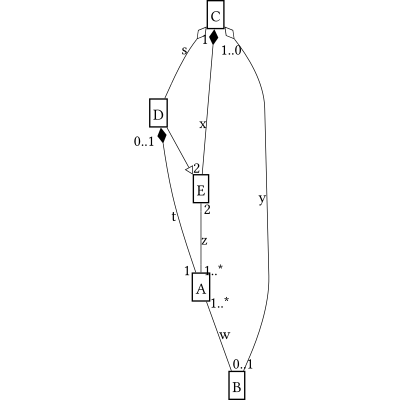
\includegraphics[min width=0.4\textwidth=0.6\textwidth,min height=0.4\textwidth=0.6\textwidth,keepaspectratio,max width=0.9\textwidth,max height=0.9\textwidth]{55/cd1f882efeb23899f5319e1c35becb46dfc9e88ddd7f53b630fc0d497cc283f32a01af83b04c596701db35357ce8aed00a3a92e08161.pdf}\end{centering}



Your answer about change 2 is correct.

The change does not repair the class diagram as it results in:



\begin{centering}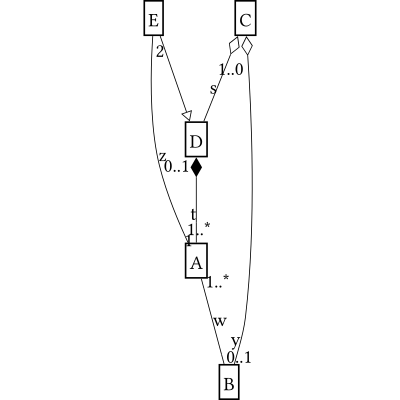
\includegraphics[min width=0.4\textwidth=0.6\textwidth,min height=0.4\textwidth=0.6\textwidth,keepaspectratio,max width=0.9\textwidth,max height=0.9\textwidth]{55/cd372dcf78cba387c70c311fa6fb5bc2294d1e800b0bb90895da49b88c5f04cb9f01af83b04c596701db35357ce8aed00a3a92e08161.pdf}\end{centering}



Your answer about change 3 is correct.

The change repairs the class diagram as it results in:



\begin{centering}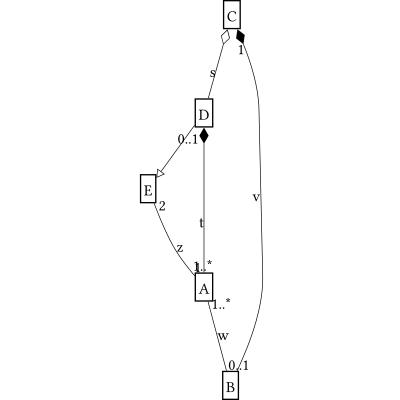
\includegraphics[min width=0.4\textwidth=0.6\textwidth,min height=0.4\textwidth=0.6\textwidth,keepaspectratio,max width=0.9\textwidth,max height=0.9\textwidth]{55/cdd57d65fcec6e477fb0e1f78931d2be37419fbfb95fca7c11558bcdc6ea2d3f9a01af83b04c596701db35357ce8aed00a3a92e08161.pdf}\end{centering}



Your answer about change 4 is not correct.

The change repairs the class diagram as it results in:



\begin{centering}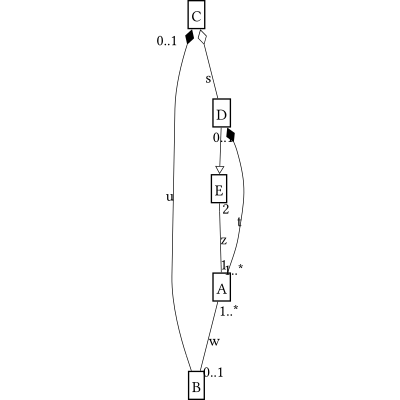
\includegraphics[min width=0.4\textwidth=0.6\textwidth,min height=0.4\textwidth=0.6\textwidth,keepaspectratio,max width=0.9\textwidth,max height=0.9\textwidth]{55/cd0a4766434bf2f8c477292745ce2f23eb3a8e30f201276bea66381532c88d1a8601af83b04c596701db35357ce8aed00a3a92e08161.pdf}\end{centering}



